% !TeX root = ../main.tex
% Add the above to each chapter to make compiling the PDF easier in some editors.

\chapter{Background}\label{chapter:background}

\section{Microcontrollers}
Since this thesis is focused on the use of WebAssembly on microcontrollers, we would like to introduce the concept and limitations shortly. A microcontroller (**MCU** for microcontroller unit) is a small computer, meant to fulfill a very specific requirement without a complex operating system. They are designed for embedded applications from implantable medical devices to toys and very prominently in IoT devices. Devices will often have multiple microcontrollers, each responsible for a particular function. A car, for example, could include, amongst others, an MCU to control the mirror adjustments, one to handle fuel injection and another one for traction control.

\begin{figure}
    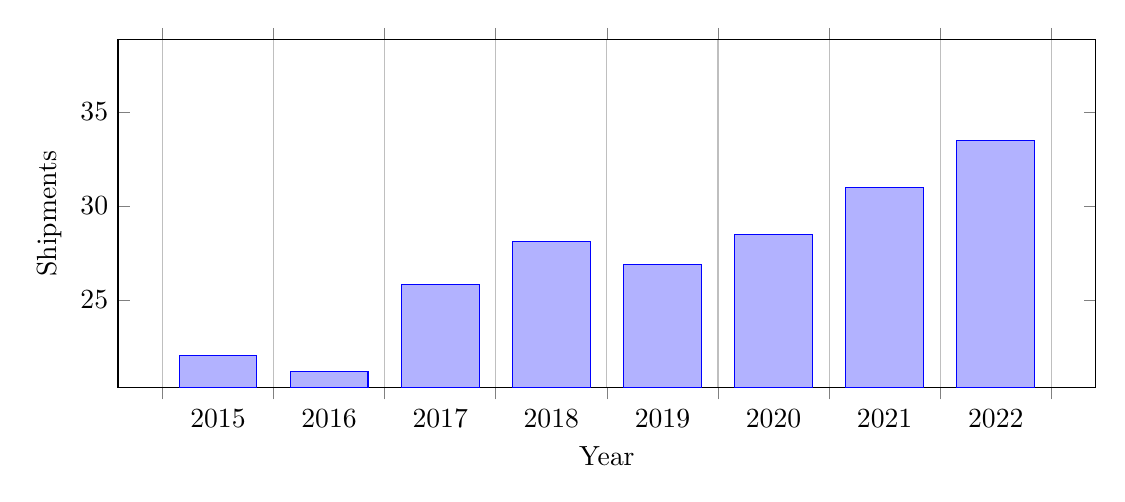
\begin{tikzpicture}
        \begin{axis}[
            x tick label style={
                /pgf/number format/1000 sep=},
            ylabel=Shipments,
            xlabel=Year,
            width=14cm,
            height=6cm,
            enlargelimits=0.05,
            ybar interval=0.7,
        ]
        \addplot 
            coordinates {(2015,22.06) (2016,21.17)
                 (2017,25.8) (2018,28.1) (2019,26.9) (2020,28.5) (2021,31) (2022,33.5) (2023,38)};
        \end{axis}
    \end{tikzpicture}
    \caption{MCU shipments worldwide from 2015 to 2023 (in billions)}
\end{figure}

Core elements of an MCU are the processor, memory, and I/O peripherals. The Processor (CPU) can be thought of as the brain of the MCU. It performs basic arithmetic, logic, and I/O operations. The memory is where any data is stored the processor needs to fulfill its tasks. Mainly there is program memory, which holds the MCUs instructions and Data memory, which servers as temporary storage while a program is executed. Lastly, the I/O peripherals are the controller's connection to the outside world; they allow the receiving and sending of information, such as receiving a signal from a switch and turning on a light in response.

\subsection{ESP32}
For this thesis, we want to specifically focus on the ESP32 system on a chip (SoC). A very popular low-cost, low power series of microcontrollers with integrated WiFi and Bluetooth. Developed by the Shanghai-based company Espressif Systems this successor to the ESP8266 offers a great platform for IoT and embedded projects\autocite{noauthor_esp32_nodate}. Compared to the MCU described before, the ESP32 has the additional processing power and I/O options that make it a great platform for developing secure IoT devices. It gained popularity fast after being released in September of 2016.

The ESP32 systems family provides an excellent base for many IoT applications. There are multiple versions available from ones very well suited for hobbyists to ones usable for industrial manufactures. With a low price point and area footprint, they still provide significant performance and many operational features\autocite{maier_comparative_2017}.

To reach price and power consumption targets, the ESP32 has significant hardware limitations. This introduces some constraints when working with the platform. The Operating system for example can hardly be called that. Compared to popular operating systems like windows and linux, the used FreeRTOS can be thought of as a thread library. This specialty will be further explained in the following passage.
\subsection{FreeRTOS}\label{subsec:freertos}
Many MCUs are used in applications where throughput is less important than a guaranteed performance. This is why the ESP32 uses FreeRTOS, a real-time operating system (RTOS) is specifically intended to be used in time-critical situations. A key characteristic of such an operating system is the predictable behavior of the scheduler, the part of the operating system that decides which task should be run by the CPU at any given time. Most schedulers allow the user to set priorities for tasks in order to decide which task should be run next.

FreeRTOS specifically is the leading RTOS amongst MCUs and is designed to be small enough to run on a microcontroller\autocite{noauthor_freertos_nodate}. Since most applications in which MCUs are used do not warrant the use of a full RTOS, FreeRTOS only provides the core scheduling functionality, timing, and synchronization primitives. It can, however, be extended by using addon components, for example, to make use of a specific networking stack. FreeRTOS also built a significant community and support for many platforms in its 15-year development.

In more recent history amazon has taken over stewardship of FreeRTOs and also offers their own extension a:FreeRTOS\autocite{lardinois_amazon_nodate}. This version additionally comes with some direct integration into amazons AWS service\autocite{noauthor_freertos_nodate-1}. It is supposed to make the development of new IoT devices easier, especially when using amazons platform for the server side processing, the core of FreeRTOS remains open soruce still.
\section{WebAssebly}
Beginning with static HTML pages, the web has since developed into a common application platform, accessible from many different devices running different operating systems. JavaScript is the only natively supported language on the web. However, even though it is universally used and made a lot of progression modern implementations, it still has some problems as a compilation target. WebAssembly addresses these issues and provides a compilation target for the web.

WebAssembly (WASM) was first announced in June 2015 and reached a cross-browser consensus in March 2017. Its goal was to provide near-native performance for browser-based applications, which could only be written in JavaScript for a long time. Since being published in March 2017, it is currently usable for about 90\% of global internet users. More recently, the interest picked up around usage outside of the browser, which is also the primary concern of this thesis.

Being meant for the web, WASM has to achieve specific goals that give the platform new properties. It has to be safe since, on the web, code is loaded mainly from untrusted sources. It has to be fast as the primary motivation to introduce WebAssembly was to provide a compile target on the web with reliable performance. Other than the usual low-level code such as regular assembly, WebAssembly has to be portable and work in all the different circumstances the web is currently used. Lastly, because the code is transmitted over the network, it has to be as small as possible to reduce bandwidth and improve latency.

WASM is a low-level binary format, designed to be a portable target for high-level languages like C\\C++ or Rust. It is executed on a stack-based virtual machine on which it executes in near-native speed due to its low-level design. Still, it runs in a memory-safe environment inside the browser and is subject to the same security policies as JavaScipt code would be. WebAssembly modules are loaded with the application and provide bindings to JavaScript that make them usable in the browser.

Together with the binary format of WebAssembly, there is a text format that defines a programming language with syntax and structure. Every WASM binary is a self-contained module with functions, globals, tables, imports, and exports. This concept provides both encapsulation and sandboxing since modules can only interact with their environment using imports, and the client can only access the specified exports. Inside the module, the code ins organized in functions that can call each other even recursively.
\subsection{WebAssembly for IoT}
While WASM is developed for the web, it carefully avoids any dependencies on the web. It is meant to be an open standard that can be embedded in a variety of ways. The goals mentioned above, which WebAssembly achieves, make it an exciting format to explore on embedded devices. Due to it's aim to be universal it would allow the use of languages on MCUs that where not previously supported and since it is already meant to be transmitted over the network, also over the air updates of code running on the controller are possible. To achieve portability, the source level interface libraries would have to map the host environments' capabilities either at build time or runtime.

While WebAssebly in an IoT context is a very promising concept it is also a brand new development. The best support for WASM right now is in the browser of course but out of browser runtimes keep surfacing, implmented in various langugaes and providing an interesting execution environment. Runtimes meant to be used on MCUs are much more rare and not as mature yet. Given the big interest in the idea though and the working groups avoidance of web depnedencies it can be assumed that this situation will change in the future.
\subsection{Interpreters}
WIth our specific usecase in mind, the WASM3 engine was chosen since it's sepcific goal is to run WebAssembly on MCUs. Other than many other engines it does not follow a jsut in time compilation pattern though, but instead acts as an interpreter. Thus we'd like to shortly introduce the concept and advantages.

Interpreters are computer programs that execute a program. They pose a different concept to compiled execution, where a program would be translated to machine code before being run directly on the CPU. While offering multiple advantages, the main drawback is the execution speed compared to native code execution, which is often slower by order of magnitude and sometimes more. The overhead is generated by the interpreter having to analyze the program code before it can be executed.

Interpreters thus offer benefits in development speed since the code does not have to be recompiled to run and in portability because the same code could be run on multiple platform-specific interpreters without the need to compile it into the native machine code of multiple platforms. For our use-case, the interpreter executes WASM instructions, allowing the dynamic loading of modules and running them in the chose environment.
\section{Microbenchmarking}
Benchmarking is any form of measurement to qualify the behavior of a system. The most obvious examples would be measuring performance, energy or memory consumption, but also relibality and temeprature stability could contribute to a benchmark. Building good bechmarks is hard, because a program has to be created that yields repeatable and consinstent results. A mejor effort in the world of microcontroller benchmarking is the EEMBC.

The embedded microprocessor banchmark consortium is an industry association that has been designing benchmarks for over 20 years. The consortium offers multiple benchmarks, all meant to cover sepcific usecases od embedded controllers from ultra-low power IoT applications, over processor performance measurements to a recent benchmark designed to assess machine learning performance.